\begin{pastexam}[label={px:gw3-096-ds-01}]{關務三等資訊處理 96 年 第一題}
（申論；20 分）

假設我們要對一組訊息 AAAAABBCCCDDDDE 進行二進位數的編碼（Code）
\begin{itemize}[leftmargin=2.2em, nosep]
\item[㈠] 若每個字元編碼為相等長度，則此訊息進行編碼後，最少需多少位元？（10 分）
\item[㈡] 若每個字元編碼為可變長度，則此訊息進行編碼後，最少需多少位元？（10 分）
\end{itemize}
\end{pastexam}

\begin{pastsoln}
答案：㈠ $45$ 位元。 ㈡ $33$ 位元（霍夫曼編碼）。

訊息共 $15$ 個字元，出現次數：A $5$、B $2$、C $3$、D $4$、E $1$。

\textbf{㈠ 等長編碼。} $5$ 種字元，每個碼要能區分 $5$ 種，碼長至少 $\lceil \lg 5 \rceil = 3$ 位元（$2$ 位元只有 $4$ 種組合，
不夠）。 所以最少 $15 \times 3 = 45$ 位元。

\textbf{㈡ 可變長度。} 為了能唯一解碼，用前置碼（prefix code，沒有一個碼是另一個碼的前綴）；總長最短的前置碼由霍夫曼
演算法求得（資結書第~19.3~節、定理~19.5）。 每次合併出現次數最小的兩個：
\begin{enumerate}
\item E(1)、B(2) 合併成 $3$。
\item C(3)、$\{E,B\}$(3) 合併成 $6$。
\item D(4)、A(5) 合併成 $9$。
\item $6$、$9$ 合併成 $15$，是根。
\end{enumerate}
\begin{center}
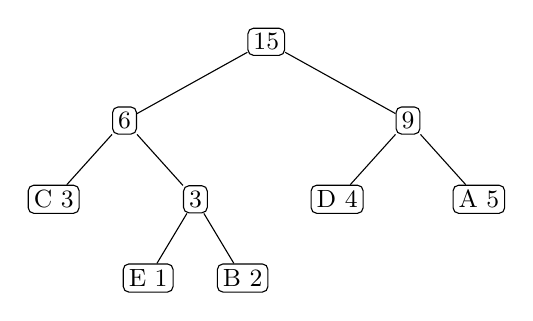
\begin{tikzpicture}[every node/.style={draw,rounded corners=2pt,inner sep=2pt,font=\small},
  level distance=10mm, level 1/.style={sibling distance=36mm}, level 2/.style={sibling distance=18mm},
  level 3/.style={sibling distance=12mm}]
\node {15}
  child {node {6} child {node {C 3}} child {node {3} child {node {E 1}} child {node {B 2}}}}
  child {node {9} child {node {D 4}} child {node {A 5}}};
\end{tikzpicture}
\end{center}
左邊記 $0$、右邊記 $1$，得到的碼：C $00$、E $010$、B $011$、D $10$、A $11$。 總長
\[
5 \cdot 2 + 2 \cdot 3 + 3 \cdot 2 + 4 \cdot 2 + 1 \cdot 3 = 10 + 6 + 6 + 8 + 3 = 33 \text{ 位元},
\]
也等於每次合併的和 $3 + 6 + 9 + 15 = 33$（資結書引理~19.6）。 比等長編碼省了 $12$ 位元。 平手時（第 2 步 C 和
$\{E,B\}$ 都是 $3$）怎麼選，碼會不同，但總長一定是 $33$。
\end{pastsoln}
